\documentclass[11pt,a4paper]{article}
\usepackage[margin=2.4cm]{geometry}
\usepackage{amsmath,amssymb}
\usepackage{graphicx}
\usepackage{booktabs,multirow,array,tabularx}
\usepackage{xcolor}
\usepackage{xurl}
\usepackage[hidelinks]{hyperref}
\usepackage{tikz}
\usetikzlibrary{arrows.meta,positioning,fit,calc}
\usepackage{enumitem}
\usepackage{caption}
\captionsetup{font=small,labelfont=bf}
\setlist{itemsep=2pt,topsep=4pt}

\newcommand{\nue}{\ensuremath{\nu_e}}
\newcommand{\numu}{\ensuremath{\nu_\mu}}
\newcommand{\code}[1]{\texttt{\small #1}}
\newcommand{\best}[1]{\textbf{#1}}

\title{\textbf{A Charge + Light Self-Supervised Foundation Model\\ for MicroBooNE LArTPC Open Data}\\[4pt]
\large Technical Note --- Round 1}
\author{Haiwang Yu\thanks{Prepared with the assistance of Claude (Anthropic). Code: \url{https://github.com/HaiwangYu/fm4npp-lartpc}, branch \code{round1-prototype}, package \code{multi-modal-qlmatch/qlfm}. Review thread: GitHub issue \#1.}}
\date{October 16, 2026}

\begin{document}
\maketitle

\begin{abstract}
\noindent
We present a prototype multi-modal foundation model for liquid-argon TPC data that takes reconstructed charge hits and PMT light as a single token sequence. A Transformer backbone is pretrained without labels, by masked autoencoding, on 831k MicroBooNE overlay events. We then evaluate it on four downstream tasks with small task heads: hit-level and event-level neutrino/cosmic separation, flavor classification ($\nu_\mu$CC/$\nu_e$CC/NC) and neutrino-energy regression. Labeled-data fractions range from 0.1\% to 100\%.

Pretraining clearly helps when labels are scarce. With 0.1\% labels, the fine-tuned charge-plus-light model beats training from scratch on every task; for example, hit-level F1 is 0.77 versus 0.22.

Adding light improves every task and is decisive for neutrino/cosmic separation: event-level AUC is 0.97 versus 0.65 for charge only.

At fixed compute, a 6.6M-parameter model saturates at about 10\% of the pretraining data. A 21M-parameter model trained twice as long improves all probes, and with it more pretraining data helps consistently. On neutrino/cosmic separation the best models clearly beat the Pandora and flash-PE reference baselines: hit F1 0.95 versus 0.63, and event AUC 0.999 versus 0.82 and 0.91.

We also show that, with fixed-grid charge patches, the masked-reconstruction target is not learnable unless each patch is positioned at its charge centroid. Round 1 used about 29 Polaris node-hours.
\end{abstract}

\tableofcontents
\vspace{6pt}

%=====================================================================
\section{Introduction and goals}
%=====================================================================
Foundation models (FMs) learn reusable representations from unlabeled data. Small task-specific heads are then trained on top, as in language and vision. Recent neutrino and nuclear-physics work applies this idea to 3D charge point clouds~\cite{polarmae,panda,pandav2} and to collider TPC space-points~\cite{fm4npp}.

A LArTPC records two correlated measurements of the same event:
\begin{itemize}
  \item ionization charge on the wire planes;
  \item scintillation light on the PMTs.
\end{itemize}
Classical reconstruction relates the two explicitly, for example through Wire-Cell's many-to-many charge--light matching~\cite{wcqlmatch,wcgeneric}. This round tests whether a single self-supervised backbone can learn these correlations, and the physics they carry, directly from paired charge and light.

Round 1 asks three questions, using the MicroBooNE public open samples~\cite{ubopendata}:
\begin{description}
  \item[Q1] Does SSL pretraining help? We compare a downstream model trained from scratch with a frozen FM plus head and with a fine-tuned FM, across label budgets.
  \item[Q2] Does light help? We compare charge-only (C) with charge+light (CL) inputs.
  \item[Q3] How does the FM scale with the amount of pretraining data (1\%, 10\%, 50\%, 90\%)?
\end{description}

The compute allowance was 100 node-hours on the Polaris \code{debug}/\code{debug-scaling} queues, which have a 1-hour walltime. Section~\ref{sec:conclusion} gives the stopping criterion.

%=====================================================================
\section{Data and tasks}
%=====================================================================
\subsection{Samples, preprocessing and splits}
We use two NoWire HDF5 samples:
\begin{itemize}
  \item the BNB inclusive overlay (Zenodo 8370883): 753{,}467 events, 195\,GB;
  \item the \nue-CC overlay (Zenodo 7261921): 18 of 20 files, 77{,}340 events.
\end{itemize}
Together they give 830{,}807 events. Both samples are GENIE+Geant4 neutrinos overlaid on real off-beam cosmic data, so cosmic hits carry no MC truth.

The HDF5 tables are converted into a column-wise, memory-mappable cache (146\,GB for the inclusive sample):
\begin{itemize}
  \item \textbf{per hit:} plane, wire, time, integral, rms; truth (deposited neutrino energy and category); and a Pandora $\nu$-slice flag, used only as a baseline;
  \item \textbf{per optical hit:} channel, time and PE;
  \item \textbf{per event:} truth, the Pandora score and the largest beam flash.
\end{itemize}

Splits are assigned by a hash of (run, subrun). Overlays that share an off-beam cosmic frame therefore stay in one partition. The pretraining subsets (1/10/50/90\% of all events) and the label pools (0.1/1/10/100\% of train) are nested random subsets of the train partition.

\begin{table}[h]
\centering\small
\caption{Partitions of the merged corpus. Following the review decision, the \nue\ sample is mixed into every partition.}
\begin{tabular}{lrr}
\toprule
Split & Events & \nue-sample share \\
\midrule
train & 747{,}068 & 9.4\% \\
val   & 41{,}912 & 9.2\% \\
test  & 41{,}827 & 7.2\% \\
\bottomrule
\end{tabular}
\end{table}

\paragraph{Audit (inclusive sample).}
\begin{itemize}
  \item 15.4k hits per event (median).
  \item 44\% of events have the $\nu$ vertex in the active volume (AV).
  \item In 21\% of events the neutrino leaves $\le 5$ hits.
  \item The beam flash follows the neutrino interaction time by $0.478~\mu$s (5--95\%: 0.457--0.507\,$\mu$s).
  \item About 1\% of optical hits fall outside the $23.4~\mu$s beam window and are dropped.
\end{itemize}

\subsection{Downstream tasks}
Table~\ref{tab:tasks} summarizes the tasks. All definitions live in \code{qlfm/data/labels.py}.

\begin{table}[h]
\centering\small
\caption{Downstream task definitions. AV = active volume; FV = fiducial volume, 3\,cm inside the AV; ``visible'' means $\ge 30$ collection-plane $\nu$ hits.}
\label{tab:tasks}
\begin{tabularx}{\textwidth}{l X l l}
\toprule
Task & Definition & Train counts & Metric \\
\midrule
T1 hit $\nu$/cosmic & Per hit: $\nu$ if the MC $\nu$-deposit exceeds 0.05\,MeV. Evaluated on events with a visible in-AV $\nu$ & $\sim$6\% $\nu$ hits & charge-wtd F1 \\
T2 event $\nu$/cosmic & 0 = no $\nu$ charge ($\le$5 $\nu$ hits); 1 = visible in-AV $\nu$; 2 = out-of-AV $\nu$ leaving $>5$ hits & 142k/333k/241k & AUC (1 vs 0) \\
T3 flavor & FV + visible: \numu CC / \nue CC / NC & 200k/68k/49k & macro-F1 \\
T4 energy & FV + visible + CC; regress $\log E_\nu$ & 268k & resolution$^\dagger$ \\
\bottomrule
\multicolumn{4}{l}{\footnotesize $^\dagger$ Half the 16--84\% interval of $(E_\mathrm{pred}-E_\mathrm{true})/E_\mathrm{true}$.}
\end{tabularx}
\end{table}

\paragraph{Reference baselines.}
\begin{itemize}
  \item \textbf{T1:} Pandora hits in the slice with the highest \code{nu\_score}.
  \item \textbf{T2:} Pandora's maximum \code{nu\_score} gives AUC 0.82; the beam-flash PE in 3--6\,$\mu$s gives AUC 0.91.
\end{itemize}

%=====================================================================
\section{Model}
%=====================================================================
Figure~\ref{fig:model} shows the architecture.

\begin{figure}[h]
\centering
\resizebox{\textwidth}{!}{%
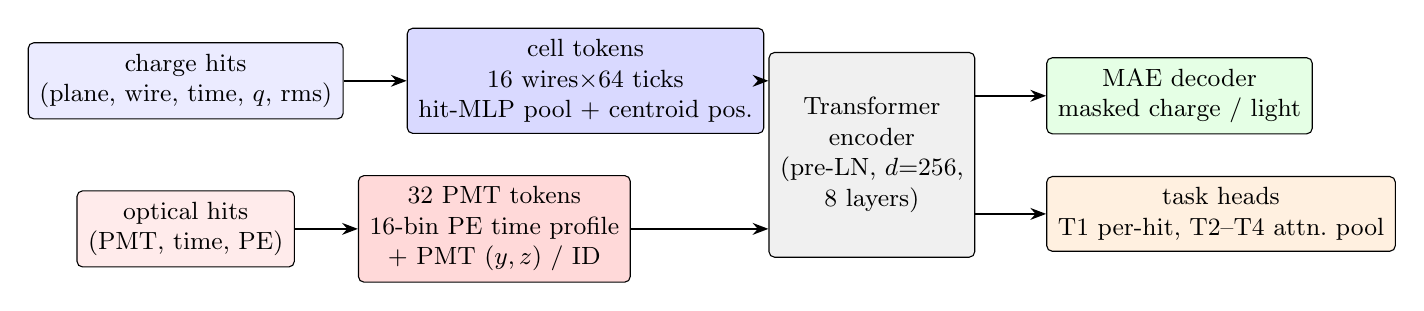
\begin{tikzpicture}[
  box/.style={draw, rounded corners=2pt, align=center, font=\small, minimum height=0.9cm, inner sep=4pt},
  arr/.style={-{Stealth[length=2mm]}, thick}]
\node[box, fill=blue!8] (hits) {charge hits\\(plane, wire, time, $q$, rms)};
\node[box, fill=red!8, below=0.9cm of hits] (oph) {optical hits\\(PMT, time, PE)};
\node[box, fill=blue!15, right=0.8cm of hits] (ctok) {cell tokens\\16 wires$\times$64 ticks\\hit-MLP pool + centroid pos.};
\node[box, fill=red!15, right=0.8cm of oph] (ltok) {32 PMT tokens\\16-bin PE time profile\\+ PMT $(y,z)$ / ID};
\node[box, fill=gray!12, minimum height=2.6cm, right=0.9cm of $(ctok.east)!0.5!(ltok.east)$] (enc) {Transformer\\encoder\\(pre-LN, $d{=}256$,\\8 layers)};
\node[box, fill=green!10, right=0.9cm of enc, yshift=0.75cm] (dec) {MAE decoder\\masked charge / light};
\node[box, fill=orange!12, right=0.9cm of enc, yshift=-0.75cm] (heads) {task heads\\T1 per-hit, T2--T4 attn.\ pool};
\draw[arr] (hits) -- (ctok); \draw[arr] (oph) -- (ltok);
\draw[arr] (ctok.east) -- (enc.west |- ctok.east); \draw[arr] (ltok.east) -- (enc.west |- ltok.east);
\draw[arr] (enc.east |- dec.west) -- (dec.west); \draw[arr] (enc.east |- heads.west) -- (heads.west);
\end{tikzpicture}}
\caption{Architecture. Charge cells and PMTs become 256-dimensional tokens in a shared space, with a modality embedding added to each. Pretraining uses the MAE decoder; downstream tasks attach small heads to the encoder.}
\label{fig:model}
\end{figure}

\subsection{Tokenization}
\paragraph{Charge tokens.}
\begin{itemize}
  \item Each wire plane is divided into $16$-wire $\times$ $64$-tick cells, about $4.8\times3.5$\,cm$^2$. Every occupied cell becomes one token.
  \item This gives about 2.0k tokens per event (median; 99th percentile 3.4k; capped at 4096).
  \item A shared per-hit MLP takes each hit's relative wire, relative time, $\log q$ and rms. Its outputs are max- and mean-pooled over the cell and concatenated with the cell's hit count and total charge.
  \item The token's position is its charge-weighted centroid in physical units (drift $x$ and wire coordinate, in cm). It is encoded by 10-octave Fourier features, plus an embedding of the centroid's offset inside the cell, plus a plane embedding.
\end{itemize}

\paragraph{Light tokens.}
\begin{itemize}
  \item There are 32 tokens per event, one per PMT.
  \item Each carries $\log(1+\mathrm{PE})$ in 16 time bins spanning 0--24\,$\mu$s, binned more finely around the expected neutrino flash, plus the total PE.
  \item The position is encoded by Fourier features of the PMT $(y,z)$ plus a PMT-ID embedding.
\end{itemize}

A modality embedding is added to every token. The charge-only model simply has no light tokens. Tokenization runs on the GPU from raw hits.

\subsection{Backbone}
The encoder is a pre-LN Transformer~\cite{preln}: 8 layers, token width $d{=}256$, 8 heads of dimension 32, and MLP hidden size 1024. It has 6.6M parameters. Pre-LN applies LayerNorm to the input of each sublayer and leaves the residual path untouched:
\[
x \leftarrow x + \mathrm{Attn}(\mathrm{LN}(x)), \qquad x \leftarrow x + \mathrm{MLP}(\mathrm{LN}(x)).
\]
This trains more stably than the original post-LN form. Downstream heads read the encoder output without a final LayerNorm, following~\cite{polarmae}. Events are packed into variable-length sequences and processed with FlashAttention-2~\cite{flashattn2}.

\subsection{Pretraining objective}
We use a multi-modal masked autoencoder~\cite{mae,multimae}.

\paragraph{Charge.}
\begin{itemize}
  \item 60\% of the charge tokens are masked.
  \item Half of the masked budget comes from 256-tick drift-time strips masked jointly on all three planes, so the model cannot copy a hidden region from another plane's view.
  \item The decoder ($d{=}192$, 3 layers) predicts, for each masked cell, a $4\times8$ in-cell charge sub-grid plus the cell's $\log$ hit count and $\log$ total charge. Each target dimension is standardized per batch.
\end{itemize}

\paragraph{Light.} Each event uses one of three masking modes:
\begin{itemize}
  \item 50\% of the PMTs are masked, with probability 0.4;
  \item all 32 PMTs are masked, with probability 0.4. This makes the task \emph{charge$\to$light} prediction, a learned stand-in for a photon library combined with flash matching;
  \item nothing is masked, with probability 0.2.
\end{itemize}

\paragraph{Schedule.} Training runs for 17k steps at a global batch of 256 events, on one Polaris node (4$\times$A100) in about 45\,min. We use AdamW with learning rate $1.5\times10^{-4}$, 5\% warmup, cosine decay and bf16. The step count is the same for every pretraining fraction.

\subsection{A fixed-grid MAE target needs patch centres}\label{sec:centroid}
In the first version, each charge token was positioned at its cell centre. The masked-charge loss never beat a per-dimension mean predictor, while the light reconstruction learned normally.

\paragraph{Diagnosis.}
\begin{itemize}
  \item A single-batch overfit test and a target-leak test confirmed that the code was wired correctly.
  \item Fourier, learned-grid and combined position encodings all failed in the same way.
  \item A non-neural baseline settled the question. Predicting a masked cell's (hit count, total charge) as the average over its visible neighbours is \emph{worse} than predicting the global mean, for $8\times32$, $16\times64$ and $32\times128$ cells.
\end{itemize}
Tracks cross a fixed grid at arbitrary offsets: a corner clip gives 1--2 hits, while a central crossing gives about 16. Unless the model knows where the track passes through the cell, the cell's content is not predictable.

\paragraph{Fix.} Following Point-MAE~\cite{pointmae} and PoLAr-MAE~\cite{polarmae}, tokens are positioned at their charge centroid, together with the centroid's offset inside the cell. With this change the held-out masked-charge error drops from 0.97--0.99 to $0.61\times$ the mean baseline.

\subsection{Heads and adaptation modes}
\paragraph{Heads.}
\begin{itemize}
  \item \textbf{Event-level tasks (T2--T4):} an attentive-pooling head, in which 4 learned queries cross-attend to all tokens, followed by an MLP. It has about 0.5M parameters.
  \item \textbf{Hit-level task (T1):} a per-hit MLP that takes the hit embedding concatenated with the contextual feature of its token.
\end{itemize}

\paragraph{Modes.}
\begin{itemize}
  \item \emph{scratch}: random initialization; everything is trained.
  \item \emph{frozen}: the backbone is fixed and only the head is trained.
  \item \emph{FT}: everything is trained, with layer-wise learning-rate decay 0.75.
\end{itemize}

\paragraph{Training and evaluation.}
\begin{itemize}
  \item Each run uses one GPU, batch size 32, and $\mathrm{clip}(30\ \text{epochs}, 400, 15000)$ steps.
  \item Early stopping uses a random validation subset.
  \item Tests use a random test subset of up to 20k events (3k for T1).
  \item Label budgets $\le$1\% are run with three seeds.
\end{itemize}

%=====================================================================
\section{Experiments}
%=====================================================================
\begin{table}[h]
\centering\small
\caption{Experiment overview. Total compute was about 29 node-hours (\code{sbank}: 29.6 charged on suballocation \code{debug}). Jobs were submitted by a queue-aware feeder; several single-GPU runs shared each node through a lock-based task queue.}
\begin{tabularx}{\textwidth}{l X r}
\toprule
ID & Content & Runs \\
\midrule
E1 & Scratch sanity checks of the label pipelines (inclusive-only corpus) & 4 \\
E2 & Pretraining of FM-C and FM-CL on 90\% of the data & 2 \\
E3 & \{scratch, frozen, FT\} $\times$ \{C, CL\} $\times$ \{0.1, 1, 10, 100\}\% labels $\times$ 4 tasks; 3 seeds at $\le$1\% & 192 \\
E4 & Pretraining of FM-C and FM-CL on 1/10/50\% of the data; frozen probes at 1\% and 10\% labels & 6 + 48 \\
E5 & Checks: learning-rate scan for scratch-C; layer decay 0.9 for hit fine-tuning & 8 \\
E6 & Larger model (21M parameters, 2$\times$ steps), FM-CL on 10\% and 90\%; frozen and FT probes & 2 + 24 \\
\bottomrule
\end{tabularx}
\end{table}

%=====================================================================
\section{Results}
%=====================================================================
\subsection{Label efficiency and the value of light (E3)}

\begin{figure}[h]
\centering
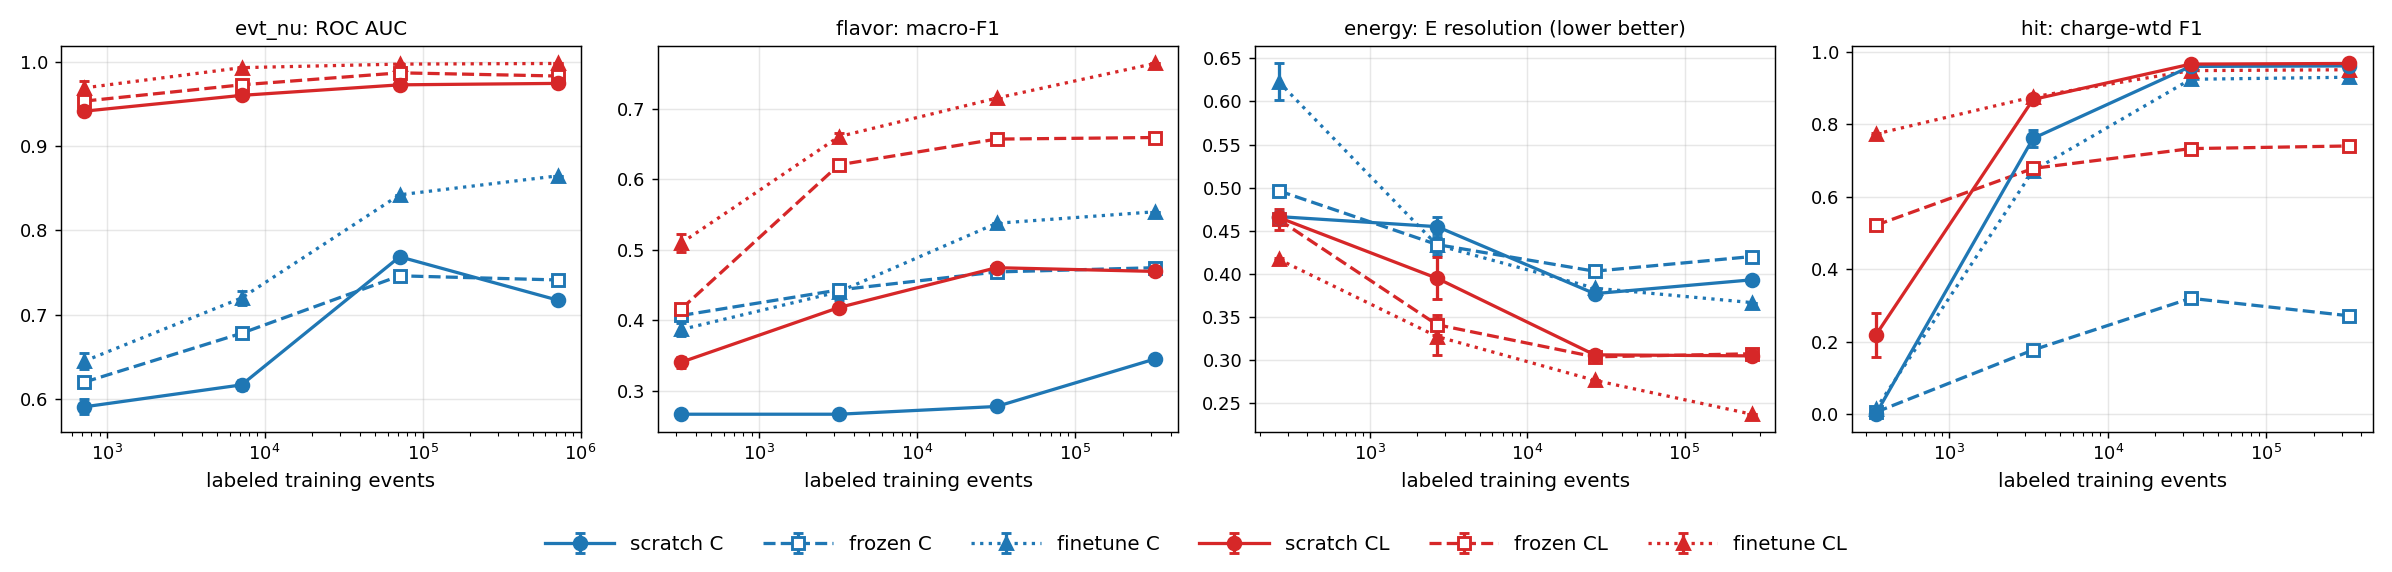
\includegraphics[width=\textwidth]{../figures/e3_label_efficiency.png}
\caption{Test metrics versus the number of labeled training events. Colour: input (blue C, red CL). Marker and line: mode (scratch $\circ$ solid, frozen $\square$ dashed, FT $\triangle$ dotted). Error bars show the seed spread at $\le$1\% labels.}
\label{fig:e3}
\end{figure}

\begin{table}[h]
\centering\small
\caption{E3 test metrics at 0.1\,/\,1\,/\,10\,/\,100\% labels. Entries at $\le$1\% are the mean of three seeds; the seed spread is typically $\le 0.01$. For T4, lower is better.}
\label{tab:e3}
\begin{tabular}{llcc}
\toprule
Task (metric) & Mode & C & CL \\
\midrule
\multirow{3}{*}{T2 event $\nu$ (AUC)} & scratch & 0.59 / 0.62 / 0.77 / 0.72 & 0.94 / 0.96 / 0.97 / 0.98 \\
 & frozen & 0.62 / 0.68 / 0.75 / 0.74 & 0.95 / 0.97 / 0.99 / 0.98 \\
 & FT & 0.65 / 0.72 / 0.84 / 0.87 & \best{0.97 / 0.99 / 1.00 / 1.00} \\
\midrule
\multirow{3}{*}{T3 flavor (macro-F1)} & scratch & 0.27 / 0.27 / 0.28 / 0.35 & 0.34 / 0.42 / 0.48 / 0.47 \\
 & frozen & 0.41 / 0.44 / 0.47 / 0.47 & 0.42 / 0.62 / 0.66 / 0.66 \\
 & FT & 0.39 / 0.44 / 0.54 / 0.55 & \best{0.51 / 0.66 / 0.72 / 0.77} \\
\midrule
\multirow{3}{*}{T4 energy (resolution)} & scratch & 0.47 / 0.46 / 0.38 / 0.39 & 0.47 / 0.40 / 0.31 / 0.31 \\
 & frozen & 0.50 / 0.43 / 0.40 / 0.42 & 0.46 / 0.34 / 0.30 / 0.31 \\
 & FT & 0.62 / 0.43 / 0.38 / 0.37 & \best{0.42 / 0.33 / 0.28 / 0.24} \\
\midrule
\multirow{3}{*}{T1 hit (charge-wtd F1)} & scratch & 0.00 / 0.76 / 0.96 / 0.96 & 0.22 / 0.87 / \best{0.97 / 0.97} \\
 & frozen & 0.01 / 0.18 / 0.32 / 0.27 & 0.52 / 0.68 / 0.73 / 0.74 \\
 & FT & 0.01 / 0.67 / 0.92 / 0.93 & \best{0.77 / 0.88} / 0.95 / 0.95 \\
\bottomrule
\end{tabular}
\end{table}

\paragraph{Best model (FT-CL, 100\% labels).}
\begin{itemize}
  \item \textbf{T2:} AUC 0.999. Signal efficiency is 0.997 at 95\% background rejection and 0.973 at 99\%. The in-AV versus out-of-AV AUC is 0.96, and the 3-class macro-F1 is 0.82.
  \item \textbf{T3:} \numu CC efficiency/purity 0.88/0.92; \nue CC 0.80/0.72 (AUC 0.96); NC 0.65/0.63.
  \item \textbf{T4:} resolution 23.7\%, bias $-2.5\%$.
  \item \textbf{T1:} charge-weighted efficiency/purity 0.948/0.953. Pandora reaches 0.78/0.56 on the same events.
\end{itemize}

\paragraph{Interpretation.}
\begin{itemize}
  \item \textbf{Q1: pretraining helps most with few labels.} The advantage shrinks as labels grow.
  \begin{itemize}
    \item On T1, scratch catches up by 1\% labels and is slightly ahead at $\ge$10\%.
    \item On the event-level tasks, FT-CL stays ahead even at 100\%. Scratch is limited there by the downstream budget ($\le$15k steps, less than one epoch), so part of that gap is undertraining.
  \end{itemize}
  \item \textbf{The frozen CL backbone is a strong feature extractor for event-level tasks.} It matches or beats scratch at every budget on T2--T4.
  \item \textbf{Frozen features are weak for per-hit labels.} The per-hit embedding receives no direct pretraining signal.
  \item \textbf{Q2: light dominates neutrino/cosmic separation.}
  \begin{itemize}
    \item Charge-only models must find a small interaction among roughly 26 cosmic muons.
    \item The in-time PMT pattern points directly to the neutrino. This is the learned counterpart of charge--light matching.
    \item Light also improves flavor and energy.
  \end{itemize}
  \item \textbf{Charge-only scratch fails on event-level tasks} at every tested learning rate (E5). Fine-tuning the same architecture from the C foundation model succeeds: flavor 0.54--0.55 and T2 AUC 0.84--0.87 at 10--100\% labels.
  \item \textbf{No sample-origin shortcut is seen for flavor.} The \nue CC efficiency on inclusive-sample \nue\ events ($n{=}79$) is equal to or higher than on \nue-sample events: 0.86 versus 0.80 for FT-CL.
\end{itemize}

\subsection{Pretraining-data scaling (E4, E6)}

\begin{figure}[h]
\centering
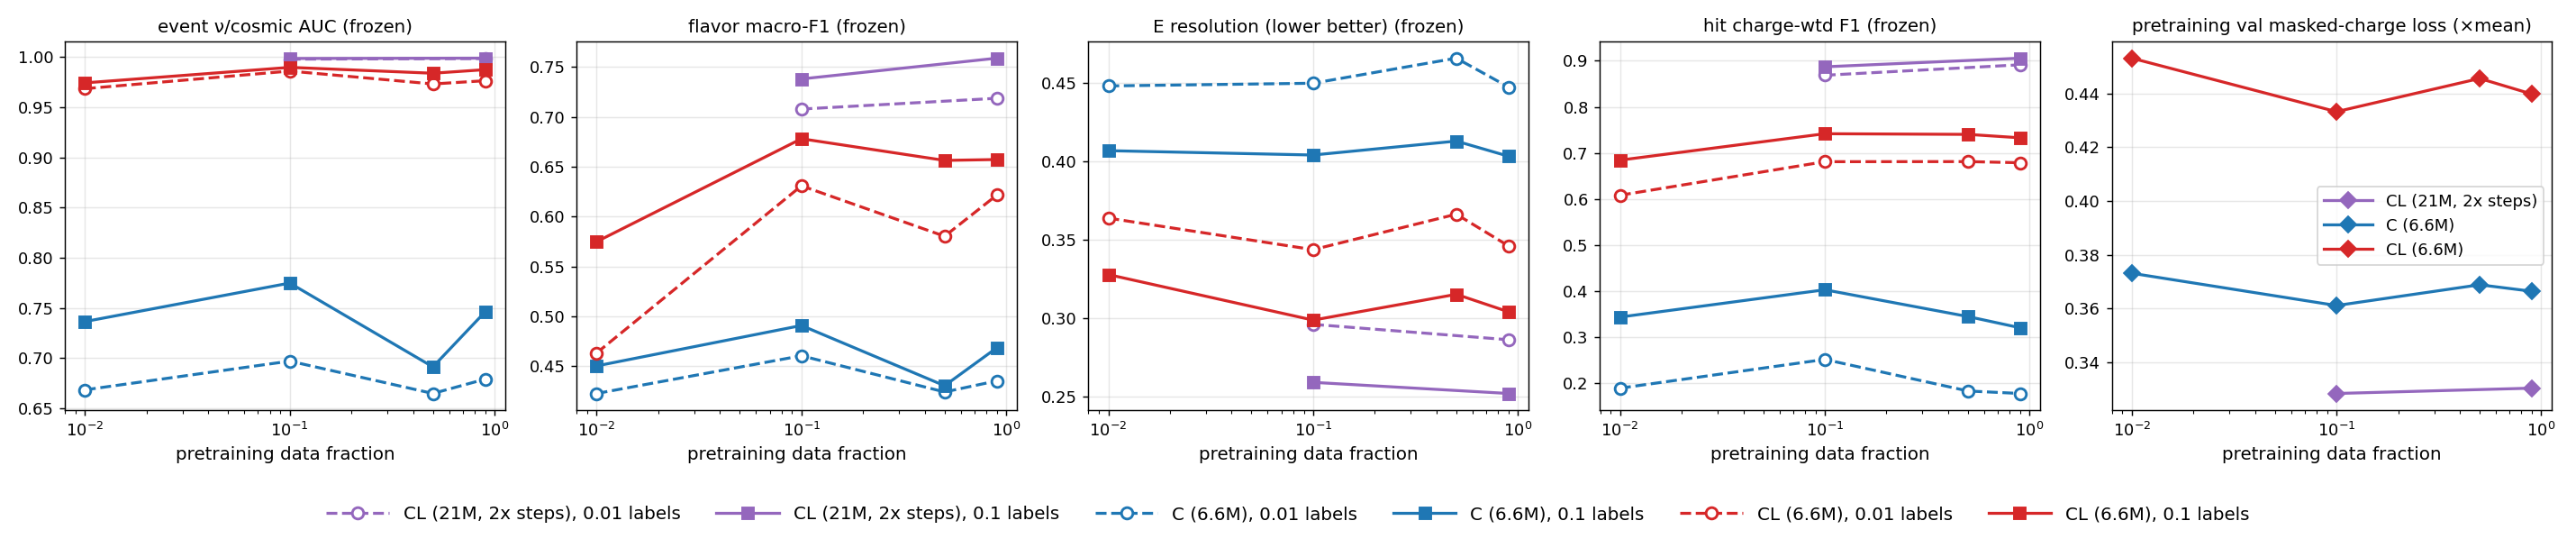
\includegraphics[width=\textwidth]{../figures/e4_scaling.png}
\caption{Frozen-probe test metrics and pretraining validation masked-charge loss versus the pretraining-data fraction. Red and blue: 6.6M CL and C models at fixed compute (17k steps). Purple: 21M CL model at $2\times$ steps. Open circles with dashed lines: 1\% labels; filled squares with solid lines: 10\% labels.}
\label{fig:scaling}
\end{figure}

\paragraph{Small model at fixed compute (E4).}
\begin{itemize}
  \item CL improves from 1\% to 10\% of the pretraining data. At 1\% labels: flavor $0.46\to0.63$, T1 $0.61\to0.68$, T4 $0.36\to0.34$, T2 $0.968\to0.986$.
  \item Above 10\% the probes are flat within single-seed jitter of $\pm$0.02--0.04. C is flat throughout.
  \item The pretraining validation loss has the same shape: CL 0.453, 0.433, 0.446, 0.440; C 0.373, 0.361, 0.369, 0.366.
  \item Every run sees the same 4.4M events. With 10\% of the data (83k events, about 53 epochs), the 6.6M-parameter model already saturates.
\end{itemize}

\paragraph{Larger model (E6).} We pretrain a CL model with $d{=}384$, 12 layers and 6 heads (21M parameters) for 34k steps (about 8.7M events) on 10\% and on 90\% of the data.

\begin{table}[h]
\centering\small
\caption{Pretraining validation loss, in units of the mean-predictor baseline.}
\begin{tabular}{llccc}
\toprule
Model & Data & Masked charge & Masked light & Charge$\to$light \\
\midrule
S (6.6M) & 10\% & 0.433 & 0.448 & 0.559 \\
S (6.6M) & 90\% & 0.440 & 0.446 & 0.556 \\
M (21M, $2\times$ steps) & 10\% & 0.328 & 0.431 & 0.539 \\
M (21M, $2\times$ steps) & 90\% & 0.330 & 0.413 & 0.512 \\
\bottomrule
\end{tabular}
\end{table}

\begin{table}[h]
\centering\small
\caption{CL probe test metrics for the small (S) and large (M) models at 10\% and 90\% pretraining data. Bold marks where the 90\% model beats the 10\% model.}
\label{tab:e6}
\begin{tabular}{lcccc}
\toprule
Probe & S 10\% & S 90\% & M 10\% & M 90\% \\
\midrule
T2 AUC, frozen, 1\%\,/\,10\% labels & 0.986 / 0.990 & 0.976 / 0.987 & 0.998 / 0.999 & 0.998 / 0.999 \\
T2 AUC, FT, 1\% labels & --- & 0.993 & 0.998 & 0.999 \\
T3 macro-F1, frozen, 1\%\,/\,10\% & 0.631 / 0.678 & 0.622 / 0.657 & 0.708 / 0.738 & \best{0.719 / 0.759} \\
T3 macro-F1, FT, 1\% & --- & 0.663 & 0.724 & \best{0.741} \\
T4 resolution, frozen, 1\%\,/\,10\% & 0.344 / 0.299 & 0.346 / 0.304 & 0.296 / 0.259 & \best{0.286 / 0.252} \\
T4 resolution, FT, 1\% & --- & 0.307 & 0.292 & \best{0.274} \\
T1 F1, frozen, 1\%\,/\,10\% & 0.681 / 0.742 & 0.678 / 0.733 & 0.869 / 0.887 & \best{0.891 / 0.906} \\
T1 F1, FT, 1\% & --- & 0.875 & 0.925 & \best{0.943} \\
\bottomrule
\end{tabular}
\end{table}

\paragraph{What E6 shows.}
\begin{itemize}
  \item \textbf{Capacity and compute dominate at this scale.} Going from S to M improves every probe: frozen T1 F1 by $+0.15$ to $+0.19$, frozen T3 macro-F1 by $+0.08$ to $+0.10$, and T4 resolution by about $-0.05$.
  \item \textbf{Frozen M features rival a fully trained small model.} At 10\% labels, frozen M reaches T3 0.759 and T4 0.252. The small model fine-tuned on all labels reaches 0.765 and 0.237.
  \item \textbf{More pretraining data now helps.} With M, 90\% beats 10\% in all 9 non-saturated comparisons (T3 $+0.011$ to $+0.021$; T4 $-0.007$ to $-0.018$; T1 $+0.018$ to $+0.022$). With S, the same comparisons were flat or reversed.
  \item \textbf{The data benefit shows up in the light objectives.} Charge$\to$light improves from 0.539 to 0.512, while the masked-charge loss is unchanged. The extra data mainly sharpens the learned charge--light correspondence.
  \item These are single seeds. The evidence is the consistent sign across all 9 comparisons, not the size of any single difference.
\end{itemize}

\subsection{Checks (E5)}
\begin{itemize}
  \item \textbf{Scratch-C learning rate.} At 10\% labels, learning rates $10^{-4}$ and $10^{-3}$ give flavor F1 0.277 and 0.267 and T2 AUC 0.69 and 0.56. The default $3\times10^{-4}$ gives 0.277 and 0.77. The scratch failure is not a learning-rate artifact.
  \item \textbf{Hit fine-tuning with layer decay 0.9} (default 0.75).
  \begin{itemize}
    \item At 10\% labels: C 0.952 (was 0.924) and CL 0.960 (was 0.948), level with scratch (0.959/0.966).
    \item At 0.1\% labels: CL 0.788 (was 0.773).
    \item A decay of 0.9 is recommended for dense tasks.
  \end{itemize}
\end{itemize}

%=====================================================================
\section{Conclusion of round 1}\label{sec:conclusion}
%=====================================================================
The round was to stop once the performance was decent and the three comparisons made physical sense, or once further iteration stopped improving the results. That point has been reached:
\begin{enumerate}
  \item Pretraining clearly beats scratch in the low-label regime, and the advantage narrows as labels grow. For per-hit labels it disappears by about 1\% labels, once fine-tuning uses a sensible layer decay.
  \item Charge+light is better than charge only on every task, and decisively so for neutrino/cosmic separation. The learned charge$\to$light prediction is non-trivial.
  \item Pretraining-data scaling is limited by compute and capacity for the 6.6M model. It reappears consistently with a larger model trained for longer.
  \item On neutrino/cosmic separation, the best models clearly beat the Pandora and flash-PE reference baselines.
\end{enumerate}
Further gains are expected from scale, from the pretraining objective and from hit-level design. These are round-2 topics (Section~\ref{sec:next}).

%=====================================================================
\section{Limitations}
%=====================================================================
\begin{itemize}
  \item \textbf{Overlay data only.} There is no beam-on or beam-off sample. The T2 negatives are overlay events in which the neutrino left no charge.
  \item \textbf{Beam-window light only} ($23.4~\mu$s). This is not Wire-Cell's full 4.8\,ms charge--light matching.
  \item \textbf{Single seeds} at 10\% and 100\% labels and in E4/E6. Differences below about 0.02 are not significant on their own.
  \item \textbf{Fixed downstream budget.} At large label budgets, scratch is not trained to convergence.
  \item \textbf{Small models and budget.} The models (6.6M and 21M parameters) and the few-million-event pretraining budget were set by the 100 node-hour allowance.
  \item \textbf{Non-natural T3 class proportions.} The \nue\ sample is mixed into all splits.
  \item \textbf{Operational label thresholds.} For example, the hit-level $\nu$ threshold of 0.05\,MeV.
\end{itemize}

%=====================================================================
\section{Next steps}\label{sec:next}
%=====================================================================
\begin{enumerate}
  \item \textbf{Hit-level representations.} Add a per-hit pretraining signal: hit-level masked prediction or dense self-distillation~\cite{panda,sonata}. Also try finer cells.
  \item \textbf{Latent self-distillation objective.} An iBOT/JEPA-style objective~\cite{ijepa} compared with MAE at matched compute.
  \item \textbf{Scaling.} Grow model size and compute together, with more seeds, and add the 1\% and 50\% points for the M model.
  \item \textbf{Backbone ablation.} FM4NPP-style per-hit tokens with a Mamba2 backbone~\cite{fm4npp}.
  \item \textbf{Physics realism.} Beam-off samples; interaction-level (slice) heads; a comparison with Wire-Cell's generic neutrino selection~\cite{wcgeneric} at matched efficiency.
\end{enumerate}

\section*{Reproducibility}
\begin{itemize}
  \item \textbf{Code:} \url{https://github.com/HaiwangYu/fm4npp-lartpc}, branch \code{round1-prototype}.
  \item \textbf{Main entry points:} \code{qlfm.data.convert}, \code{scripts/make\_splits.py}, \code{qlfm.train\_pretrain}, \code{qlfm.train\_downstream}, \code{scripts/make\_tasks.py}, \code{scripts/feeder.sh}, \code{scripts/summarize.py} and \code{scripts/plot\_scaling.py}.
  \item \textbf{Outputs:} on Polaris under \url{/lus/eagle/projects/neutrinoGPU/yuhw/fm4npp-lartpc-work/}.
  \item \textbf{Companion documents:} a Markdown version of this note with the same content (\url{docs/technote-round1.md}) and a working log of decisions and findings (\url{docs/round1-log.md}).
\end{itemize}

\begin{thebibliography}{99}\small
\bibitem{ubopendata} G.~Cerati (for MicroBooNE), \emph{MicroBooNE public data sets: a collaborative tool for LArTPC software development}, arXiv:2309.15362; data DOIs 10.5281/zenodo.8370883 and 10.5281/zenodo.7261921.
\bibitem{wcqlmatch} MicroBooNE Collaboration, \emph{Neutrino event selection in the MicroBooNE LArTPC using Wire-Cell 3D imaging, clustering, and charge-light matching}, JINST 16 (2021) P06043, arXiv:2011.01375.
\bibitem{wcgeneric} MicroBooNE Collaboration, \emph{Cosmic ray background rejection with Wire-Cell LArTPC event reconstruction in the MicroBooNE detector}, arXiv:2101.05076.
\bibitem{mae} K.~He et al., \emph{Masked autoencoders are scalable vision learners}, arXiv:2111.06377.
\bibitem{pointmae} Y.~Pang et al., \emph{Masked autoencoders for point cloud self-supervised learning}, arXiv:2203.06604.
\bibitem{polarmae} \emph{Particle trajectory representation learning with masked point modeling} (PoLAr-MAE), arXiv:2502.02558.
\bibitem{multimae} R.~Bachmann et al., \emph{MultiMAE: multi-modal multi-task masked autoencoders}, arXiv:2204.01678.
\bibitem{fm4npp} \emph{FM4NPP: a scaling foundation model for nuclear and particle physics}, arXiv:2508.14087.
\bibitem{panda} \emph{Panda: self-distillation of reusable sensor-level representations for high energy physics}, arXiv:2512.01324.
\bibitem{pandav2} \emph{Panda Diplomacy: foundation model pre-training across particle imaging detectors}, arXiv:2609.00611.
\bibitem{sonata} X.~Wu et al., \emph{Sonata: self-supervised learning of reliable point representations}, arXiv:2503.16429.
\bibitem{ijepa} M.~Assran et al., \emph{Self-supervised learning from images with a joint-embedding predictive architecture}, arXiv:2301.08243.
\bibitem{preln} R.~Xiong et al., \emph{On layer normalization in the Transformer architecture}, arXiv:2002.04745.
\bibitem{flashattn2} T.~Dao, \emph{FlashAttention-2: faster attention with better parallelism and work partitioning}, arXiv:2307.08691.
\end{thebibliography}

\end{document}
